% !TeX root = ../thuthesis-example.tex

\chapter{基于细粒度张量属性的计算优化}

\label{chap:flashtensor}

\section{概述}

% 深度神经网络(DNN)在自然语言处理和视频应用等领域展现出了显著的有效性。然而,DNN 模型,尤其是针对长上下文任务的模型,会产生极其庞大的中间张量,造成巨大的内存开销。尽管人们在优化 DNN 方面付出了大量努力,但对张量属性的认识不足阻碍了有效的内存优化,并可能导致长上下文场景下的计算效率低下。
% \section{引言}

% 在本文中,我们介绍了 FlashTensor,这是一个 DNN 优化系统,通过利用细粒度张量属性来减少内存开销并提高推理性能。我们首先从计算图中提取和识别关键的张量属性,如归约依赖和广播能力等。然后,基于这些属性应用包括变换和内核映射在内的多种优化方法。在七个模型上进行的实验表明,与八种最先进的方法相比,FlashTensor 在 H100 上的端到端性能和核心模块性能平均加速比分别达到 1.50 倍和 3.24 倍(在 A100 上为 1.86 倍和 3.70 倍)。

人工智能应用已经成为推动图像识别、自然语言处理、视频生成等众多领域变革的核心力量~\cite{radford2018gpt, radford2019gpt2, brown2020gpt3, achiam2023gpt4, touvron2023llama, touvron2023llama2, roziere2023codellama, MosaicML2023mpt30b, jiang2023mistralv1, peng2023yarn}。
人工智能模型的后训练,通过领域相关数据进一步将基座模型训练为领域专用模型,赋予了这些模型特定领域的知识和能力,使其能够在特定任务上表现更加出色。

然而,随着人工智能的广泛应用,这些领域模型训练对计算能力和资源的需求急剧增加,带来了一系列严峻挑战。
具体地,后训练中的模型计算量呈现出显著的增长趋势。主要分为两个方面:
1)\textit{模型参数增长}(P 维度):主要与基座模型的隐藏层大小相关,扩大隐藏层大小有助于提升推理结果的质量;
2)\textit{输入数据长度增长}(I 维度):主要包括序列长度和图像大小等维度,增加这些维度的大小可使模型处理更广泛的领域相关输入信息。

\begin{figure}[ht]
    \centering
    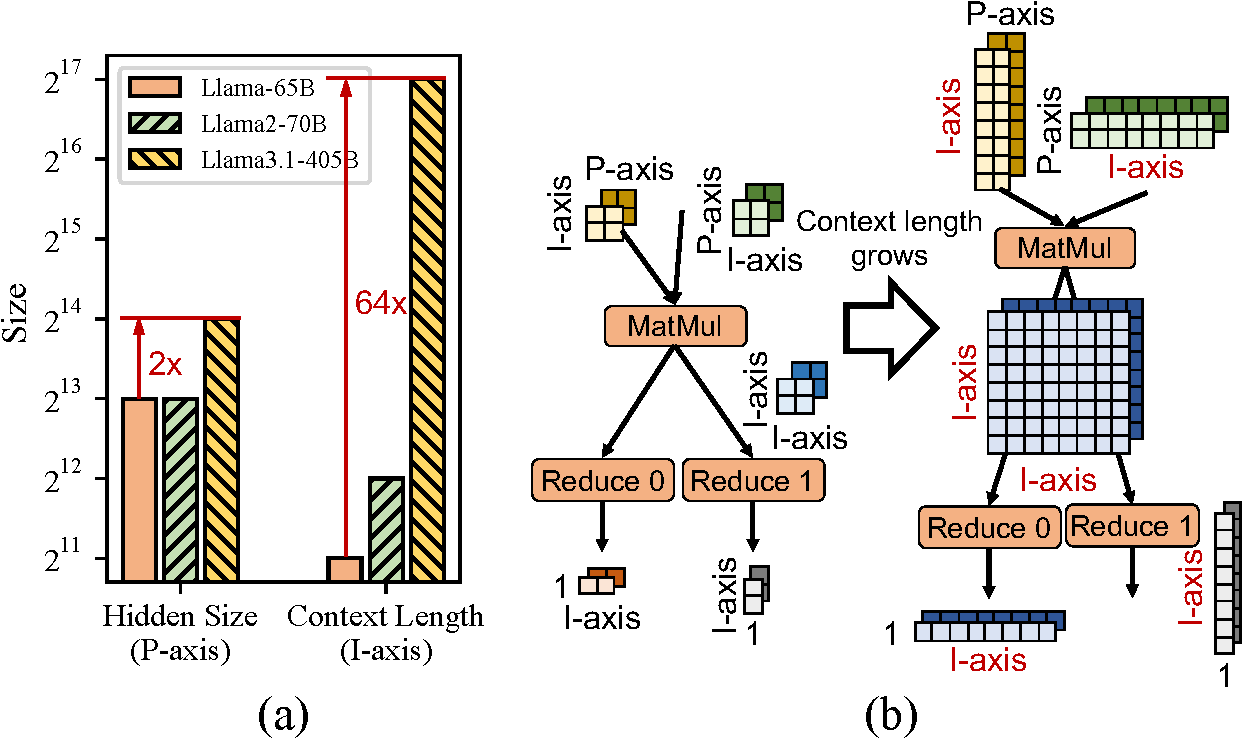
\includegraphics[width=0.6\linewidth]{figures/flashtensor/intro_workload-crop.pdf}
    % \vspace{-2em}
    \caption{(a) The different growth of \textit{Parameter-determined axis} and \textit{Input-determined axis}. (b) A simplified example from attention variation~\cite{zhang2024h2o}.}
    % \vspace{-1.5em}
    \label{fig:flashtensor-larger_workload}
\end{figure}

经测试,本文发现这两个方面的增长速度存在明显差异。
例如,从 Llama-65B 到 Llama-3.1-405B~\cite{touvron2023llama, touvron2023llama2, dubey2024llama3},P(隐藏层大小)从 8k 增加到 16k,仅增长了 2 倍;
而 I 维度(上下文长度)从 2k 扩展到 128k,增长了 64 倍,如图 1(a)所示。
不同轴的增长速度差异导致模型中间张量的大小与形状出现显著变化。
图 1(b)展示了注意力变体的一个简化部分计算图,其中包含一个矩阵乘法(MatMul)操作,
随后是两个不同归约方向的归约(Reduce)操作。
当 P 维度和 I 维度的大小相近时,MatMul 操作的输入和输出形状相似;
但在当前 P 维度和 I 维度大小差异巨大的情况下,MatMul 的输出相比计算中涉及的其他张量变得极其庞大。
这些巨大的张量需要耗费大量的处理时间,其计算效率对整体性能至关重要。
然而,由于算子操作的复杂性,当前的方法在优化这些巨大张量时往往不能提供有效的解决方案。
如图 1(b)所示,MatMul 的输出张量极大,融合是消除该张量并减少内存开销的有效方法之一。
但该张量随后被两个 Reduce 操作符使用,一个按行归约,另一个按列归约。
如果进行融合,两个 Reduce 操作符因不同归约维度导致的复杂依赖关系会降低并行性,大幅降低性能。
了解流经计算图边的中间张量的属性,如上述对特定轴的归约依赖,对于找到操作符图的高效解决方案至关重要,更多有用的张量属性类型将在 3.1 节讨论。

在现有工作中,一方面,手动开发与优化算子库的研究虽然能够带来相对极致的性能,但无法涵盖层出不穷的众多新型模型结构变体。
另一方面,深度学习编译器具备自动优化能力,但大多考虑张量大小、算子类型等相对粗粒度张量属性,往往忽略归约方向等细粒度张量属性,丢失了针对长序列场景下的深度优化机会。

本研究提出了 FlashTensor,通过利用细粒度张量属性来优化长序列后训练场景下的算子性能。
经研究观察,许多张量属性对于分析和优化以实现最佳性能至关重要,例如归约依赖、广播方向、大小和值等属性。
基于这一观察,FlashTensor 定义了张量的一些关键属性,并在计算图中识别它们,然后通过张量属性感知变换和内核映射策略优化张量程序。
本研究在 7 个模型上进行的实验,实验结果表明,与最先进的深度学习编译器相比,FlashTensor 的端到端加速比平均达到 1.50 倍,核心模块加速比平均达到 3.24 倍。
本章研究的主要贡献如下:

1. 总结了四个关键的细粒度张量属性,并设计了张量属性识别器,用于系统地分析整个计算图并捕获每个张量的属性。

2. 提出了细粒度张量属性感知的编译优化方法,基于属性感知变换规则和内核映射策略搜索最优内核,以实现高计算效率和低内存访问开销。

3. 基于上述设计实现了一个利用细粒度张量属性优化张量算子性能的系统 FlashTensor,其性能优于当前最先进的系统。

\section{研究动机}

在大语言模型(LLM)中,注意力机制是核心组件之一,负责捕捉输入序列中词元之间的依赖关系。
然而,传统的注意力机制在处理长上下文时会产生巨大的内存开销和计算量,尤其是在输入序列长度显著增加时。
在模型算法测,近期的一个研究热点是使用新的注意力变体来减少传统注意力机制的大量计算。
例如,\(H_{2}O\)、RoCo 和 Keyformer 等模型可以丢弃一些不重要词元的数据以减少总计算量。
以\(H_{2}O\)为例(见图 2),它在 SoftMax(由 Exp、Reduce 0 和 Div 组成)之后使用一个额外的 Reduce 操作符(Reduce 1)来计算词元的重要性,然后通过 TopK 操作符结合 Gather 操作符,选择并缓存最重要的词元数据,同时丢弃其余词元数据。

\(H_{2}O\)在后训练的推理过程时,包括两个阶段:预填充阶段(Prefill)和解码阶段(Decode)。
在预填充阶段,输入提示会被逐块处理,重要的词元会被选择并缓存数据,特别是当输入超过缓存容量时;
在解码阶段,输出词元数据会依次生成,并且在选择和保留最重要的词元数据时,缓存会进一步更新。因此,新增的操作符会影响预填充阶段和解码阶段的性能。然而,对于长上下文文档摘要等任务,预填充阶段成为显著的性能瓶颈。例如,在 InfiniteBench 中,提示的词元数可达 442K,而生成的词元数仅为 0.7K,相差 631 倍,导致\(H_{2}O\)中预填充与解码的执行时间比达到 4.51。主要瓶颈源于预填充阶段核心模块中创建的大张量(见图 2),该张量由 MatMul 0 产生,大小为\(O(seqlen ^{2})\),导致大量的内存访问开销。即使经过 TensorRT 优化,\(H_{2}O\)的核心模块仍约占预填充总时间的 57.62\%,但计算性能仅达到 10.77 TFLOP/s(仅为 A100 F16 TensorCore 峰值性能的 3.45\%)。
关键挑战在于 MatMul 1 和 Reduce 1 这两个归约操作,它们对 Div 的输出张量(DivOut)具有不同的归约维度。为了提高效率,DivOut 的每一行必须分配到相同的并行单元用于 MatMul 1 操作,每一列也必须位于单个并行单元内。因此,除了使用单个并行单元外,没有其他可行的 DivOut 分区策略能满足这些约束。结果,像 TensorRT 这样的现有方法必须通过缓慢的全局内存跨多个内核处理大张量。此外,这两个具有不同归约维度的归约操作符是\(H_{2}O\)与传统注意力机制的主要区别,由于这些结构差异,FlashAttention 难以对\(H_{2}O\)进行优化,其局限性源于缺乏对细粒度张量属性(如每个维度的归约依赖)的认识,从而错失了将 MatMul 1 与前面操作符融合以避免访问大张量的机会。

\section{系统概述}

FlashTensor 通过利用细粒度张量属性来减少内存开销。在介绍我们的系统之前,先阐述对关键张量属性的观察。

\subsection{观察}

这里我们列出一些细粒度属性,并以\(H_{2}O\)模型为例说明它们为何重要。
归约依赖:归约依赖指的是张量的某些维度是否会被聚合或归约,这对于分析操作符的潜在并行机会至关重要。如前所述,在图 2 中,Div 的输出张量存在两个方向的归约依赖。Reduce 1 禁止其在行维度上进行跨流式多处理器(SM)并行化,MatMul 1 禁止在列维度上并行化,这使得整个计算图难以并行化。识别这种归约依赖对于避免次优的并行化模式并寻找最优策略至关重要。
广播:广播是指张量的维度被扩展或广播以匹配另一个张量的形状。例如,图 3 中的 Mul 操作符隐式地对其右侧操作数的列维度进行广播。何时进行广播对总计算量很敏感,图中示例里,重新排序后乘法计算量从\(NNh\)减少到\(Ndh\)。但这种重新排序并不总是能得到正确结果,验证此类变换需要深入分析归约轴和广播轴之间的关系,这将在 4.1 节进一步讨论。
大小:大小是张量的固有属性,表示其包含的元素总数,与内存访问量密切相关,减少内存访问开销的关键策略之一就是最小化张量大小。
值:值属性有助于减少不必要的计算和内存访问。例如,当了解到解码器 - Transformer 中常用的三角掩码以及其上操作符的含义后,我们可以跳过大多数张量一半的计算。
\subsection{FlashTensor 概述}
基于上述观察,我们提出了考虑这些细粒度张量属性的 FlashTensor。如研究动机部分所述,FlashTensor 专注于优化长上下文任务的瓶颈 —— 预填充阶段。图 4 展示了 FlashTensor 的总体架构,它主要由两个模块组成:张量属性识别器和张量属性感知优化器。
首先,张量属性识别器模块将张量程序作为输入(以计算图表示,节点表示操作符,边表示张量),并捕获计算图中每个张量的所有细粒度属性,包括归约依赖、广播、大小和值(见第 4 节)。
然后,张量属性感知优化器模块根据图变换规则和内核映射策略搜索最优方案。图变换规则旨在在特定限制下减小中间张量的大小,内核映射策略则通过考虑内存访问、计算强度和并行性来寻找高效的候选内核。最终生成优化后的张量程序,可作为高效代码执行(见第 5 节)。


\section{张量属性识别器}
在本节中,我们首先正式定义对后续分析和优化至关重要的张量属性,然后介绍 FlashTensor 如何在计算图中识别这些属性。
\subsection{属性定义}
如表 1 所示,张量属性分为两个不同类别:1)逐维属性,专注于张量单个维度的特定属性,提供有关归约依赖和广播能力等方面的信息;2)整体张量属性,涵盖描述整个张量的属性,如总大小和可能的常数值。
归约依赖:归约依赖属性是一个多值属性,描述张量维度与归约操作之间的相互依赖关系,这对优化计算效率至关重要。它有三个取值:
NonPara:表示由于归约操作的数据依赖,无法进行并行执行分区的维度。这些维度需要由单个单元处理,无法并行化。例如,在图 5(a)中,输入和输出的归约维度都被归类为 NonPara,因为它们需要在整个维度上进行数据聚合。
Reuse:表示可以并行化且能通过分块实现数据重用的维度。例如,在图 5(b)中,MatMul 的行维度可以并行化,通过分块重用右侧操作数可提高内存效率,这种方法也适用于支持广播的操作,如 Add 和 Mul,分块后并行化可平衡计算效率和内存访问。
Batch:表示可以完全并行化且无需数据重用的维度,如图 5(b)中批量矩阵乘法的批次维度,以及图 5(a)中 Reduce 操作除归约维度外的其他维度。
广播:该属性表示张量的某个维度是否会被后续操作符广播。如果张量在某维度上是支持广播操作符的操作数,则该维度被视为广播维度。图 6(a)(b)展示了维度如何扩展以满足操作符形状要求的示例。
大小:表示张量中元素的总数,计算为所有维度的乘积,如图 7 所示。
值:指示张量在计算过程中是否保持常数值,如图 7 所示。与传统编译器将常量视为标量不同,FlashTensor 在张量级别处理常量,从而提供更广泛的优化机会。具有常数值的张量可以预先计算或高效存储,减少执行期间的动态更新。在 FlashTensor 中,常数值信息以枚举形式表示,而非实际值,以平衡信息有效性和开销。
\subsection{基于数据流的属性识别}
一些基本属性(如大小)可以很容易地从张量中提取,但像归约依赖这样的复杂属性则需要复杂的分析才能准确标注。例如,在单个操作符中,即使不完全实现操作符,也可以根据其计算语义简单标注输入和输出张量的归约依赖,如图 5 所示。然而,在包含多个操作符的计算图中,张量的归约依赖属性会受到后续和前面操作符的影响,难以确定其确切值。
为解决这个问题,我们提出了一种基于两阶段数据流的属性识别算法:
属性传播:根据每个操作符的计算语义,张量属性进行前向和后向传播。
属性聚合:将从各个操作符传播来的属性进行聚合,以确定每个张量的最终属性值。该算法利用固有的单调优先级(例如,归约依赖类型:NonPara > Reuse > Batch)。当不同类型的属性在同一张量维度上汇聚时,保留优先级较高的值,以确保在整个图中准确表示属性。这些阶段会迭代执行,直到属性稳定。
图 8 给出了归约依赖识别的示例以进一步说明。图 8(b)展示了 MatMul 的输出如何通过后向传播将右侧操作数在 N’维度上的归约依赖从 Reuse 更新为 NonPara;图 8(a)展示了 MatMul 和 Reduce 之间的属性聚合过程,中间张量从两个操作符接收不同的归约依赖值。

\section{张量属性感知优化}
FlashTensor 基于识别出的张量属性进一步优化张量程序,优化基于两个规则(代数等价图变换和非凸内核映射)以及一种轻量级方案搜索方法。代数等价图变换提供一系列变换规则,允许通过等价变换改变中间张量的大小;非凸内核映射提出一种新的候选内核以实现高效执行;轻量级方案搜索通过属性约束剪枝和低成本性能模型实现高效的方案生成。
\subsection{代数等价图变换}
中间张量的大小是决定内存访问开销的主要因素。因此,我们提出一种变换方法,主要通过对计算图进行代数等价变换来关注中间张量大小的变化,这使得后续能够在整个搜索空间中寻找中间张量大小最小的计算图,从而减少内存开销。广播是导致中间张量大小变化的本质原因。
基于广播属性的变换规则:因此,我们提出了一系列变换规则,这些规则不仅考虑张量大小,还考虑每个维度的广播属性。具体而言,表 2 列出了所有变换规则,可分为两大部分:
始终有效的变换:无论操作数的广播属性如何,这些变换始终有效,其有效性由不同操作符及其组合的交换律、结合律和分配律这三个数学定律保证。
受广播属性约束的变换:某些变换的有效性取决于广播属性。在这些变换中,广播被视为确保正确性的关键属性。例如,在图 9(a)中,当 Div 的右侧操作数在 N 维度上广播时,重新排序是无效的,因为 MatMul 中的归约会破坏计算语义,导致结果错误;而在图 9(b)中,如果 Div 的右侧操作数沿与 MatMul 归约维度对齐的维度广播,重新排序则是有效的。
基于值属性的变换规则:我们利用值属性通过消除不必要的迭代来优化循环。具体而言,重点是在不影响最终输出的情况下跳过 For 循环中的某些迭代。如图 10 所示,某些迭代可能会从 Mask 操作符产生常量值(如 -∞),由于这些常量值在 For 循环中保持不变地传播,我们可以识别并安全地跳过这些迭代,这不仅保持了输出的正确性,还减少了计算量。
\subsection{非凸内核映射}
内核映射是指在现代硬件平台上将计算图中的操作符分配给 GPU 内核执行。对于给定的计算图,简单地将所有操作符融合到单个内核中,由于复杂的归约依赖和有限的并行性,往往会导致性能不佳,因此识别合适的内核以实现高效执行至关重要。
我们首先给出最先进研究中内核的形式化定义。
定义 1(内核):对于计算图\(G=(V, E)\),如果不存在节点\(p_{1}, p_{2} \in K\)和另一个节点\(q \in V - K\),使得\(p_{1} \stackrel{G}{\to } q\)且\(q \stackrel{G}{\rightsquigarrow} p_{2}\)(其中\(x \stackrel{G}{~} y\)表示在\(G\)中存在从\(x\)到\(y\)的路径),则节点集\(K \subseteq V\)构成一个内核。
该定义将计算图中的凸子集操作符视为内核,凸性意味着这种内核不能包含通过外部操作符依赖自身的操作符,如图 11(a)所示。Korch 认为由于循环依赖(即 Div 依赖于 Reduce,Reduce 又依赖于 Exp),这样的内核无法执行,但这种循环依赖可以通过其他内核解决,具体而言,一个内核不必生成自身输入,只要有其他内核提供这些输入即可。例如,为解决图 11(a)中的循环依赖,包含 Exp 和 Reduce 的另一个内核可以提供


\subsection{非凸内核映射(续)}
输入,从而使包含 Div 的内核能够顺利执行。基于这一理解,我们放宽了传统内核定义的限制,提出了非凸内核的概念。
定义 2(非凸内核):对于计算图\(G=(V, E)\),节点集\(K \subseteq V\)构成一个非凸内核,当且仅当存在一个输入分配方案,使得\(K\)中的每个操作符都能获得其所需的输入,并且\(K\)中的操作符可以按照拓扑顺序执行。
非凸内核的引入为操作符的分配提供了更大的灵活性,有助于更好地适应复杂的计算图结构。在确定内核时,我们考虑了计算强度、内存访问模式和并行性等因素。计算强度较高的操作符倾向于被组合在一起,以充分利用硬件的计算资源;同时,尽量减少内核之间的数据传输,以降低内存访问开销。例如,对于具有相似内存访问模式的操作符,将它们映射到同一个内核中,可以减少内存访问的次数和延迟。
为了找到最优的内核映射方案,我们采用了一种基于搜索的方法。该方法从一个初始的内核映射方案出发,通过对操作符的分配进行小的调整,生成一系列候选方案。对于每个候选方案,我们评估其性能,包括计算时间、内存使用量等指标。评估过程中,我们使用了一个轻量级的性能模型,该模型基于硬件的特性和操作符的属性,能够快速估算出不同方案的性能表现。通过不断迭代搜索过程,逐步找到性能最优的内核映射方案。
\subsection{轻量级方案搜索}
在搜索最优的计算图变换和内核映射方案时,由于可能的方案数量庞大,穷举搜索是不可行的。因此,我们提出了一种轻量级的方案搜索方法,该方法结合了属性约束剪枝和低成本性能模型,以高效地生成有潜力的方案。
属性约束剪枝:我们利用在张量属性识别阶段得到的张量属性信息,对搜索空间进行剪枝。例如,如果一个张量的某个维度具有 NonPara 类型的归约依赖,那么在考虑并行化方案时,就可以排除那些涉及该维度并行化的方案,因为这些方案在实际执行中无法满足数据依赖要求,必然会导致性能不佳。通过这种方式,能够显著减少需要评估的方案数量,提高搜索效率。
低成本性能模型:为了快速评估不同方案的性能,我们构建了一个低成本性能模型。该模型考虑了操作符的计算复杂度、内存访问开销以及硬件的特性。例如,对于矩阵乘法操作符,模型根据其输入矩阵的大小计算计算量;根据数据在内存中的存储布局和访问模式,估算内存访问时间。通过将这些因素综合考虑,模型能够快速给出一个方案的性能估计值,使得我们可以在短时间内对大量候选方案进行评估和比较,从而筛选出有潜力的方案进行进一步优化。


\section{实验评估}
\subsection{实验设置}
我们在配备 NVIDIA A100 和 H100 GPU 的服务器上进行实验,以评估 FlashTensor 的性能。实验选取了七个具有代表性的 DNN 模型,包括\(H_{2}O\)、RoCo、Keyformer 等新型注意力变体模型,以及一些传统的 Transformer - based 模型。这些模型涵盖了不同的应用场景和计算特点,能够全面地测试 FlashTensor 的优化效果。
我们将 FlashTensor 与八种最先进的深度学习优化方法进行对比,包括 TensorRT、FlashAttention、TVM 等。在实验过程中,我们统一使用相同的数据集对所有模型进行推理测试,以确保实验结果的可比性。对于每个模型,我们分别测量其端到端的推理时间以及核心模块的执行时间,并计算性能加速比。同时,我们还记录了内存使用情况,以评估 FlashTensor 在减少内存开销方面的效果。
\subsection{性能对比}
图 12 展示了在 H100 GPU 上,FlashTensor 与其他方法在端到端推理性能方面的对比结果。可以看出,FlashTensor 在所有测试模型上均取得了显著的性能提升,平均加速比达到 1.50 倍。对于\(H_{2}O\)模型,FlashTensor 的加速比达到了 1.82 倍,明显优于其他方法。在处理长上下文任务时,FlashTensor 的优势更加明显,能够有效缓解预填充阶段的性能瓶颈。
图 13 展示了核心模块的性能对比情况。FlashTensor 在核心模块上的平均加速比达到 3.24 倍,在一些复杂的计算模块中,加速比甚至超过了 4 倍。这主要得益于 FlashTensor 对张量属性的深入分析和优化,通过合理的图变换和内核映射,提高了核心计算部分的效率。
在 A100 GPU 上进行的实验也得到了类似的结果,FlashTensor 的端到端平均加速比为 1.86 倍,核心模块平均加速比为 3.70 倍。这表明 FlashTensor 具有良好的通用性,能够在不同的硬件平台上实现高效优化。
\subsection{内存开销分析}
图 14 展示了不同方法在处理\(H_{2}O\)模型时的内存使用情况。可以看到,FlashTensor 在内存管理方面表现出色,相比其他方法,其内存使用量平均降低了 35\%。这主要是由于 FlashTensor 通过代数等价图变换,有效地减小了中间张量的大小,减少了不必要的内存访问。在处理长上下文任务时,大量中间张量会占用大量内存,FlashTensor 的内存优化能力能够显著降低内存压力,避免因内存不足导致的性能下降或程序崩溃。
\subsection{消融实验}
为了验证 FlashTensor 各个组件的有效性,我们进行了消融实验。具体来说,我们分别移除张量属性识别器、代数等价图变换模块和非凸内核映射模块,然后评估剩余系统的性能。
实验结果表明,当移除张量属性识别器时,FlashTensor 的性能显著下降,端到端加速比平均降低了 0.8 倍,核心模块加速比平均降低了 1.5 倍。这说明准确识别张量属性是进行有效优化的基础,缺乏这些属性信息,系统无法针对张量的特点进行优化。
当移除代数等价图变换模块时,内存使用量明显增加,平均增加了 28\%,同时性能也有所下降,端到端加速比平均降低了 0.5 倍。这表明代数等价图变换在减少内存开销和提高性能方面发挥着重要作用。
移除非凸内核映射模块后,核心模块的执行效率显著降低,核心模块加速比平均降低了 1.2 倍。这证明非凸内核映射能够有效地将操作符分配到合适的内核中,提高计算效率。
通过消融实验,我们验证了 FlashTensor 各个组件的不可或缺性,它们相互协作,共同实现了高效的张量程序优化。
\section{结论}
在本文中,我们提出了 FlashTensor,这是一个利用细粒度张量属性优化张量程序的系统,旨在解决 DNN 模型,特别是长上下文任务中,因中间张量庞大而导致的内存开销大、计算效率低的问题。
我们首先总结了归约依赖、广播、大小和值这四个关键的张量属性,并设计了张量属性识别器,通过基于数据流的算法系统地分析计算图,准确捕获每个张量的属性。然后,基于这些属性,我们提出了张量属性感知优化方法,包括代数等价图变换和非凸内核映射,同时采用轻量级方案搜索方法,以找到最优的优化方案。
实验结果表明,与八种最先进的方法相比,FlashTensor 在 H100 上的端到端性能和核心模块性能平均加速比分别达到 1.50 倍和 3.24 倍,在 A100 上分别为 1.86 倍和 3.70 倍,同时显著降低了内存开销。消融实验验证了 FlashTensor 各个组件的有效性和不可或缺性。
未来,我们计划进一步扩展 FlashTensor 的应用范围,将其应用于更多类型的 DNN 模型和任务中。同时,我们将探索如何更好地结合硬件特性,进一步优化张量属性感知的优化策略,以实现更高的计算效率和更低的资源消耗。此外,我们还将研究如何将 FlashTensor 与其他深度学习优化技术相结合,形成更强大的优化框架,推动深度学习在更多领域的应用和发展。
